\chapter{Badane funkcje układu}

\section{Obsługa SSH}
\label{sec:ssh}
Po połączeniu układu z komputerem przez interfejs USB, możliwe jest otworzenie konsoli komunikacji przy użyciu protokołu transmisji szeregowej. Komunikacja odbywa się z prędkością 115200 bodów, ośmioma bitami danych, jednym bitem stopu i bez bitu parzystości.

Komunikacja przy użyciu transmisji szeregowej jest jednak ograniczona do sytuacji, w których możliwy jest bezpośredni dostęp do układu. Ponadto, nie zapewnia wysokiej przepustowości transmisji czy możliwości przesyłu plików. Z tych powodów, korzystne staje się wykorzystanie protokołu \emph{SSH} do nawiązania komunikacji sieciowej.
Omawiany protokół wspierany jest przez zdecydowaną większość dystrybucji systemu Linux i nie wymaga dodatkowej konfiguracji na etapie budowania systemu. Połączenie odbywa się przy użyciu poniższego polecenia.

\begin{lstlisting}[breaklines=true]
ssh root@(*@\textit{}adres-ip-urządzenia}@*)
\end{lstlisting}

Domyślne hasło administratora w przypadku dystrybucji \emph{PetaLinux} to \texttt{root}. Może być ono zmienione na etapie konfiguracji systemu.


\begin{lstlisting}[breaklines=true]
petalinux-config -c rootfs
Petalinux RootFS Settings ---> Root password
\end{lstlisting}

Aby uprościć proces logowania, wykorzystać można mechanizm wymiany kluczy, zapewniany przez protokół.

\begin{lstlisting}[breaklines=true]
ssh-copy-id -i ~/.ssh/id_rsa.pub root@(*@\textit{adres-ip-urządzenia}@*)
\end{lstlisting}

Umożliwia to logowanie bez konieczności podania hasła użytkownika. Skonfigurowany w opisany sposób, protokół daje dostęp do pełnego zbioru narzędzi, w tym zdalnej obsługi konsoli użytkownika, przesyłania plików, tunelowania portów czy zdalnego montowania systemów plików.
\section{FPU i technologia NEON}
\label{sec:arm-neon}
Układ \emph{ZYBO} wyposażony jest w koprocesor arytmetyczny oraz wspiera polecenia wykorzystujące technologię NEON. \cite{neon-home} Elementy te pozwalają na zwiększenie wydajności projektowanych aplikacji w przypadku, gdy wykonywane operacje wymagają przeprowadzania obliczeń na liczbach zmiennoprzecinkowych lub działań wektorowych.

Koprocesor arytmetyczny, FPU (ang. \emph{floating-point unit}), to układ działający we współpracy z jednostką procesora, dedykowany do wykonywania obliczeń na liczbach zmiennoprzecinkowych. Wykorzystanie dedykowanego układu pozwala na zwiększenie szybkości wykonywania operacji arytmetycznych, pierwiastkowania i przesunięć bitowych. W przypadku braku dedykowanego układu FPU, konieczne jest symulowanie jego działania przez wykonywanie większej liczby operacji na liczbach całkowitych, co wiąże się ze spadkiem wydajności.

Technologia NEON pozwala na rozszerzenie puli rozkazów procesora ARM o polecenia wykorzystujące architekturę SIMD zdefiniowaną przez taksonomię Flynna.\cite{Flynn1972}

SIMD (ang. \emph{Single Instruction streams, Multiple Data streams}) to klasa systemów, które pozwalają na przetwarzanie wielu strumieni danych na podstawie jednego strumienia instrukcji. Zastosowania tej architektury obejmują zagadnienia, w których dla wielu wartości wejściowych konieczne jest wykonanie tej samej operacji. Cechę tę posiada wiele operacji związanych z przetwarzaniem sygnałów i obrazów, w tym  wyznaczanie wartości szybkiej transformaty Fouriera, implementacje filtrów FIR i IIR czy operacje skalowania, rotacji i filtracji uśredniającej obrazu.

Rozpatrzono możliwość wykorzystania architektury NEON w zagadnieniach przetwarzania sygnałów. Działanie testowano na podstawie programu wyznaczającego wartość iloczynu skalarnego dwóch wektorów zadanej długości. Porównano trzy implementacje algorytmu, którego kod źródłowy zawarto w dodatku \ref{cha:neon-source}.
Wykorzystano implementację bazową oraz z wykorzystaniem poleceń dostępnych w architekturze NEON i porównano wyniki z implementacją zaprojektowaną w asemblerze.

Implementacja w architekturze NEON wykorzystuje dedykowane funkcje, udostępnione w bibliotece \texttt{arm\_neon.h}, które mają na celu maksymalne zwiększenie wydajności aplikacji. W przypadku pozostałych implementacji, wykorzystywane są polecenia wykonywane na koprocesorze VFP (ang. \emph{Vector Floating-Point}). VFP pozwala na wykonanie tej jednej instrukcji dla wektora danych wejściowych. Układ ten nie należy do rodziny SIMD i wykonuje instrukcje sekwencyjnie, w przeciwieństwie do architektury NEON.


Wyniki testów wydajności zebrano w tabeli \ref{tab:neon-time-results}.

\begin{table}[h]
	\caption{Wyniki testu wydajnościowego.}
	\centering
	\label{tab:neon-time-results}
	\begin{tabular}{|l|l|l|l|}
		\hline
		\multicolumn{4}{|c|}{Bez optymalizacji} \\ \hline
		Implementacja & min {[}s{]} & max {[}s{]} & średnio {[}s{]} \\ \hline
		Bazowa & 0,4266 & 0,4339 & 0,4296 \\ \hline
		NEON & 0,1103 & 0,1108 & 0,1105 \\ \hline
		ASM & 0,4082 & 0,4086 & 0,4083 \\ \hline
		\multicolumn{4}{|c|}{Z optymalizacjami} \\ \hline
		Bazowa & 0,1080 & 0,1152 & 0,1092 \\ \hline
		NEON & 0,1088 & 0,1147 & 0,1090 \\ \hline
		ASM & 0,1087 & 0,1144 & 0,1089 \\ \hline
	\end{tabular}
\end{table}

Rozpatrzono przeprowadzenie procesu komplikacji z wyłączonymi optymalizacjami kompilatora (flaga \texttt{-O0}) oraz z włączonymi wszystkimi optymalizacjami (\texttt{-O3}).

Wykorzystane poleceń NEON wymaga użycia odpowiadających im parametrów kompilacji. Poniżej przedstawiono polecenie kompilacji testowej implementacji wykorzystującej NEON.

\begin{lstlisting}[breaklines]
arm-linux-gnueabihf-gcc -Wall -O3 -mcpu=cortex-a9 -mfpu=neon -ftree-vectorize -mvectorize-with-neon-quad -mfloat-abi=hard -ffast-math -g -c -o "src/main.o" "../src/main.c"
\end{lstlisting}

W sytuacji, gdy wyłączono optymalizacje na etapie kompilacji, zauważalny jest znaczny wzrok wydajności w przypadku wykorzystania instrukcji udostępnianych przez architekturę NEON. Pozwala ona na niemal czterokrotne zwiększenie szybkości działania programu względem pozostałych implementacji. Różnica ta zanika w przypadku wykorzystania możliwości optymalizacji kodu programu na etapie kompilacji. Różnica w szybkości wykonania programu NEON jest niewielka, jednak pozostałe implementacje zostały zoptymalizowane do stanu, w którym koszt ich wykonania porównywalny jest z implementacją w NEON.

Wyniki pozwalają wnioskować o słuszności wykorzystania instrukcji udostępnianych przez architekturę NEON ze względu na możliwy wzrost wydajności. Istotna jest jednak weryfikacja wyników i potwierdzenie poprawy działania aplikacji. W przypadku, gdy różnice między programami są niewielkie, użycie instrukcji NEON może być niekorzystne ze względu na zwiększoną latencję wykonania rozkazów.

\section{Protokół AXI}
\label{sec:axi-std}
Protokół AXI (ang. \emph{Advanced eXtensible Interface}) zdefiniowany został w specyfikacji AMBA (ang. \emph{Advanced Microcontroller Bus Architecture}) 3. W kolejnej wersji dokumentu sprecyzowano standard w najnowszej wersji - AXI4. \cite{axi-spec} Protokół wykorzystywany jest do komunikacji pomiędzy elementami układu lub modułami zbudowanymi wewnątrz logiki reprogramowalnej i jest dedykowany systemom o dużej wydajności i pracującym z wysoką częstotliwością.

Specyfikacja definiuje trzy typy interfejsu:
\begin{itemize}
	\item AXI4 - wykorzystujące technikę MMIO (ang. \emph{Memory-Mapped Input/Output}) do odwzorowania rejestrów w przestrzeni adresowej pamięci RAM i dedykowanej aplikacjom wymagającym dużej wydajności komunikacji.
	\item AXI4-Lite - uproszczona wersja protokołu, wykorzystująca MMIO i dedykowana aplikacjom o mniej rozbudowanych wymaganiach komunikacyjnych.
	\item AXI4-Stream - wersja przepływowa protokołu, nie wykorzystująca technik MMIO.
\end{itemize}

Interfejsy wykorzystujące technikę MMIO stosowane są powszechnie w zadaniach konfiguracji modułów aplikacji czy przesyłania informacji, takich jak ramka sygnału wizyjnego do pamięci procesora. Dzięki reprezentacji elementów logiki reprogramowalnej w pamięci, możliwa jest jednolita analiza działania całego systemu.

Interfejs w wersji \emph{Stream} wykorzystywany jest natomiast do przesyłania sygnału pomiędzy kolejnymi elementami układu, na przykład transmisji kolejnych pikseli obrazu pomiędzy kolejnymi składowymi algorytmu przetwarzania obrazu. Proces przesyłania danych w takiej formie charakteryzuje się większą wydajnością, analiza działania aplikacji jest jednak utrudniona ze względu na brak reprezentacji przesyłanych danych w pamięci.

Możliwe jest również połączenie obu typów interfejsu wewnątrz jednego elementu. Technika ta wykorzystana została w przypadku elementu AXI VDMA, umożliwiając manipulowanie ramkami obrazu wizyjnego przesyłanymi przy użyciu interfejsu \emph{Stream} dzięki buforowaniu w pamięci RAM. Zagadnienie to szerzej opisano w sekcji \ref{sec:axi-vdma}. Podobne techniki wykorzystano również w przypadku interfejsu Ethernet DMA, umożliwiającego komunikację przy użyciu protokołu Ethernet.

\subsection{Przebieg transakcji}

Transakcja komunikacyjna odbywa się pomiędzy dwoma urządzeniami - \emph{master} i \emph{slave}, jednak dzięki zastosowaniu elementów \emph{AXI-Interconnect} możliwe jest połączenie wielu urządzeń, co przedstawiono na schemacie \ref{fig:axi-interconnect}.

\begin{figure}[h]
	\centering
	\def\svgwidth{8cm}
	\input{img/axi-interconnect.pdf_tex}
	\caption{Schemat połączenia Interconnect w protokole AXI.}
	\label{fig:axi-interconnect}
\end{figure}


Komunikacja odbywa się przy użyciu pięciu niezależnych kanałów:
\begin{itemize}
	\item Read Address
	\item Write Address
	\item Read Data
	\item Write Data
	\item Write Response
\end{itemize}

Każdy kanał zawiera zbiór sygnałów wykorzystywanych w trakcie wymiany danych.

Transmisja rozpoczyna się od wykorzystania sygnałów \emph{valid} i \emph{ready}. Urządzenie źródłowe wymusza stan wysoki sygnału \emph{valid} i oczekuje na zmianę wartości sygnału \emph{ready} urządzenia docelowego na stan wysoki. W chwili, gdy oba sygnały znajdują się w tym stanie, właściwe dane mogą zostać przesłane z urządzenia źródłowego do docelowego. Pozwala to na przekazanie takich danych jak adres odczytu/zapisu do pamięci, odczytywanych lub zapisywanych danych i potwierdzenia zapisu. Proces nawiązania transakcji odbywa się niezależnie dla każdego wykorzystywanego kanału.

Procedura odczytu danych składa się z dwóch etapów:
\begin{enumerate}
	\item Zdefiniowanie  przez urządzenie \emph{master} adresu i parametrów transmisji danych na kanale \emph{Read Address}.
	\item Przesłanie przez urządzenie \emph{slave} jednej lub więcej wartości danych na kanale \emph{Read Data}.
\end{enumerate}

Natomiast procedura zapisu wymaga trzech etapów:
\begin{enumerate}
	\item Zdefiniowanie  przez urządzenie \emph{master} adresu i parametrów transmisji danych na kanale \emph{Write Address}.
	\item Przesłanie przez urządzenie \emph{master} jednej lub więcej wartości danych na kanale \emph{Write Data}.
	\item Przesłanie przez urządzenie \emph{slave} odpowiedzi na kanale \emph{Write Response}.
\end{enumerate}

Protokół pozwala ponadto na przesłanie do 256 wartości danych w trakcie jednej transmisji dzięki technice \emph{burst}, a transakcje odczytu i zapisu danych mogą odbywać się równolegle.

Przepływ danych w interfejsie AXI4-Stream odbywa się wyłącznie w jednym kierunku i nie jest możliwy odczyt danych przesłanych wcześniej przez urządzenie \emph{master} do \emph{slave}. Procedura ta jest podobna do transakcji zapisu, jest jednak rozszerzona o możliwość dzielenia operacji na kilka mniejszych i łączenia wielu transakcji w jedną.

\subsection{AXI DMA}
DMA (ang. \emph{Direct Memory Access}) to technika często stosowana w przypadku konieczności wykonywania operacji na pamięci RAM urządzenia z dużą częstotliwością. Wykorzystanie kontrolera DMA pozwala przeprowadzać operacje odczytu i zapisu do pamięci operacyjnej bez konieczności użycia głównej jednostki procesora. Dzięki temu, procesor odpowiada wyłącznie za skonfigurowanie kontrolera DMA i może wykonywać inne operacje w trakcie transmisji danych. Ponadto, stosowanie kontrolera DMA pozwala zwykle na uzyskanie wyższej przepustowości komunikacji z pamięcią i zmniejszenie zużycia energii. Kontroler DMA może również przeprowadzać podstawowe operacje konwersji sygnałów, na przykład, w przypadku sygnału wizyjnego, konwersję sygnałów synchronizacji obrazu. 

DMA pozwala na przesłanie wielu wartości danych w ramach jednej transakcji w trybie \emph{burst}. \emph{Master} przesyła wyłącznie adres pierwszego bajta danych, a kolejne adresy wyznaczane są w trakcie operacji przez urządzenie \emph{slave}. Wyznaczany adres może być inkrementowany, w przypadku, gdy operacja wykonywana jest w pamięci, bądź mieć stałą wartość, co ma miejsce w przypadku zapisu lub odczytu z kolejki FIFO (\emph{First In, First Out}). Interfejs pozwala również na ograniczenie dostępnej przestrzeni adresowej, w efekcie czego wartość adresu po przekroczeniu górnej granicy zakresu przyjmuje ponownie najniższą dopuszczalną wartość. Własność ta może być wykorzystana do projektowania linii buforujących.

Protokół AXI DMA wykorzystuje kolejność bitów, w której najmniej znaczący bajt umieszczony jest jako pierwszy.

Dzięki zastosowaniu techniki DMA możliwa jest konfiguracja parametrów pracy algorytmu zaprojektowanego w układzie logiki reprogramowalnej oraz obserwacja jego działania na etapie wykonania z poziomu procesora ARM. W szerszej perspektywie, pozwala to na udostępnienie interfejsu użytkownika, umożliwiającego nadzór nad pracą algorytmu, na przykład z poziomu konsoli dostępnej przez \emph{ssh} lub w formie interfejsu strony internetowej. Możliwe jest również wykorzystanie modułu umożliwiającego przesyłanie z poziomu logiki FPGA notyfikacji do procesora ARM w celu wymuszenia jego reakcji lub powiadomienia o osiągnięciu zadanego stanu, na przykład przesłanie informacji o ukończeniu iteracji algorytmu dla aktualnej ramki obrazu. Można w tym celu wykorzystać mechanizm przerwań systemowych, co szerzej opisano w sekcji \ref{sec:axi-interrupts}.

Mechanizm DMA zbadano na przykładzie projektu modułu umożliwiającego modyfikację parametrów oraz odczyt aktualnego stanu parametrów. Schemat strukturalny modułu przedstawiono na rysunku \ref{fig:axi-dma-diagram}.

\begin{figure}[h]
	\centering
	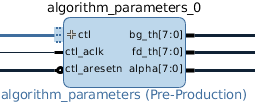
\includegraphics[]{img/algorithm-parameters.png}
	\caption{Graficzna reprezentacja modułu AXI DMA w programie Vivado.}
	\label{fig:axi-dma-diagram}
\end{figure}

Proces projektowania oraz komunikacji z modułem przedstawiono w sekcji \ref{sec:vivado-axi-dma}.

Moduł wyposażony jest w interfejs AXI, podpisany \texttt{ctl} oraz związane z nim sygnały, zegarowy - \texttt{ctl\_aclk} oraz reset - \texttt{ctl\_aresetn}. Sygnały wyjściowe pozwalają na odczyt zdefiniowanych parametrów z poziomu innych modułów logiki reprogramowalnej. Dzięki wydzieleniu modułu odpowiedzialnego za konfigurację algorytmu z części wykonującej obliczenia algorytmiczne, możliwe jest uproszczenie kodu języka opisu sprzętu związanego z każdym z modułów oraz zwiększenie czytelności schematu. Jeden moduł konfiguracyjny może być związany z kilkoma, działającymi niezależnie, modułami algorytmicznymi. Ponadto, zmiany w strukturze algorytmu są uproszczone.


\subsection{AXI Video DMA}
\label{sec:axi-vdma}
Interfejs AXI VDMA pozwala na wykorzystanie techniki DMA w przypadku aplikacji przetwarzających sygnał wizyjny.

Mechanizm \emph{Video DMA} oparty został na wykorzystaniu protokołu AXI w wersji Stream oraz Memory Mapped w połączeniu z techniką DMA do buforowania sygnału wizyjnego. 
Sygnał wizyjny przesyłany jest do modułu przy użyciu protokołu strumieniowego, gdzie następnie jest buforowany i zapisywany do komórek pamięci RAM. Zapisany obraz może być odczytany z poziomu procesora ARM. Moduł wspiera również komunikację w drugą stronę, pozwalając na odczyt obrazu z pamięci i przesłanie go dalej w postaci strumienia. Połączenie tych technik pozwala na wykorzystanie modułu do buforowania obrazu lub w celu rozdzielenia zadań algorytmicznych pomiędzy FPGA i CPU.

Moduł VDMA pozwala na zdefiniowanie do trzydziestu dwóch buforów ramek obrazu. Operacje mogą być wykonywane cyklicznie na każdym buforze lub stale na jednym z nich. Pozwala to na wielokrotną transmisję jednej klatki obrazu.

Powszechnie wykorzystywanym zastosowaniem modułu jest mechanizm potrójnego buforowania, umożliwiający zmianę częstotliwości taktowania zegara sygnału wizyjnego. Zapis i odczyt danych może odbywać się niezależnie z tego samego lub różnych buforów. Dzięki zastosowaniu trzech buforów, zagwarantować można, że zapis i odczyt danych zawsze odbywa się z niezależnych obszarów pamięci, co pozwala uniknąć zjawiska nadpisania przechowywanych danych przed ich wyświetleniem.

W niniejszej pracy rozpatrzono możliwość wykorzystania modułu VDMA w celu obsługi algorytmów wymagających kontekstu w postaci dwóch kolejnych ramek obrazu.

\section{Obliczenia równoległe}
\label{sec:openmp}

Ze względu na wykorzystanie w układzie ZYBO procesora ARM o dwóch rdzeniach, możliwe jest rozważenie zagadnienia zwiększania szybkości wykonania algorytmu przez zrówlnoleglenie obliczeń w dwóch wątkach.

Stosując prawo Amdahla, wykazać można, że maksymalne przyspieszenie, jakie można uzyskać w systemie wieloprocesorowym jest proporcjonalne do liczby elementów obliczeniowych. Zależność ta zachodzi po warunkiem, że całe zadanie może być realizowane w sposób równoległy. W przypadku omawianego procesora, spodziewać się można korzyści nie przekraczających dwukrotnego zwiększenia szybkości wykonania algorytmu.

Zagadnienia związane z obliczeniami równoległymi stanowią obszar aktualnych badań, których efekty pozwoliły na zaprojektowanie zbioru bibliotek ułatwiających wykorzystanie własności systemów wieloprocesorowych w praktyce. W ramach pracy rozważono możliwości wykorzystania wątków natywnych oraz bibliotek \emph{Intel Threading Building Blocks} i \emph{OpenMP} do budowy aplikacji wielowątkowych.

% dodatek
% linkowanie z pthread, tbb, openMP...

\subsection{Wątki natywne}

Użycie wątków natywnych wymaga wykorzystania bibliotek systemowych - w przypadku aplikacji w języku C++ działającej w systemie PetaLinux zastosować można biblioteki \texttt{<thread>} lub \texttt{<pthread.h>} wchodzące w skład bibliotek standardowych. \cite{Williams2013}
 
Wykorzystanie ich pozwala na możliwie najbardziej efektywne użycie zasobów maszyny obliczeniowej. Wymaga to jednak dużych umiejętności programisty oraz dobrej znajomości architektury docelowej oraz wykonywanego zadania. Ponadto, zastosowanie biblioteki \texttt{<pthread.h>} wymaga zgodności systemu docelowego ze standardem POSIX, natomiast w przypadku \texttt{<thread>}, konieczne jest przeprowadzenie procesu kompilacji kompilatorem zgodnym ze standardem C++11. Założenia te mogą okazać się problematyczne w przypadku konieczności migracji aplikacji na system nie spełniający opisanych wymagań.

Stosowanie wątków natywnych pozwala na budowę wielowątkowych aplikacji działających heterogenicznie. Jest to najprostszy sposób na zbudowanie programu, w którym kilka wątków odpowiada za kilka różnych zadań. Na przykład, jeden wątek może być odpowiedzialny za przeprowadzenie obliczeń algorytmicznych, drugi za obsługę interfejsu użytkownika i przygotowanie danych wejściowych do właściwych obliczeń algorytmicznych, a kolejny - za niekrytyczne operacje po zakończeniu pracy algorytmu, takie jak przesłanie wyników do bazy danych.

\subsection{Biblioteka \emph{Intel Threading Building Blocks}}

Biblioteka \emph{Intel Threading Building Blocks} stanowi zbiór narzędzi rozszerzających standard języka C++ o elementy związane z obliczeniami równoległymi. Składają się na to implementacje algorytmów równoległych, struktury danych przeznaczone do wykorzystania w systemach wielowątkowych oraz implementacje operacji atomowych i algorytmów wzajemnego wykluczania. \cite{Reinders2010}

Wykorzystanie biblioteki opiera się na zastosowaniu jej elementów na etapie powstawania aplikacji. Z tego względu, podobnie jak w przypadku wątków natywnych, konieczne jest zaprojektowanie aplikacji w sposób możliwie najlepiej wykorzystujący zalety biblioteki. Refaktoryzacja kodu istniejącego programu w taki sposób, by wykorzystać TBB może być utrudniona i ostatecznie nie pozwolić na uzyskanie zadowalających wyników.

Główną zaletą stosowania TBB jest większa skalowalność wynikowych rozwiązań. W przypadku zastosowania wątków natywnych, konieczne jest zaprojektowanie aplikacji w sposób umożliwiający wykorzystanie innej liczby wątków, gdy będzie to konieczne. W przypadku zastosowania dodatkowej biblioteki, stanowi ona warstwę abstrakcji pomiędzy programistą a warstwą obliczeniową, dzięki czemu proces możliwie najlepszej integracji aplikacji z platformą docelową odbywać się może przy niewielkiej interakcji ze strony projektanta.
Biblioteka TBB zgodna jest z ideą programowania generycznego, paradygmatu powszechnie stosowanego w aplikacjach projektowanych w języku C++. Stosowanie jej stanowi naturalne rozszerzenie możliwości tego języka i nie wymaga szerokiej wiedzy na temat architektury systemu docelowego.

\subsection{Biblioteka \emph{OpenMP}}
Biblioteka \emph{OpenMP} to interfejs programowania aplikacji pozwalający na tworzenie wieloplatformowych programów wykonywanych równolegle. Rozwiązanie to jest dedykowane aplikacjom powstającym w językach C i C++.\cite{openmp-guide}

OpenMP składa się z dyrektyw kompilatora i zbioru bibliotek, które pozwalają kształtować zachowanie programu na etapie wykonania.

Ze względu na wykorzystanie dyrektyw kompilacji, możliwa jest integracja biblioteki z istniejącą aplikacją, nie wymagając przy tym modyfikowania właściwego kodu programu. Wymaga to wyłącznie znajomości aplikacji w stopniu umożliwiającym identyfikację obszarów, których równoległe wykonanie pozwoli na osiągnięcie największych zysków.

Analogicznie jak w przypadku biblioteki TBB, zastosowanie OpenMP ma na celu zapewnienie skalowalności aplikacji i dodanie warstwy abstrakcji pomiędzy kod programu a operacje wykonywane na wątkach obliczeniowych. Obie biblioteki wyposażone są również w algorytmy równoważenia obciążenia.

Wykorzystanie biblioteki OpenMP wymaga zastosowania kompilatora wspierającego dyrektywy wchodzące w jej skład. Ze względu na specyfikę stosowania części interfejsu biblioteki - w formie komentarzy do właściwego kodu aplikacji - możliwa jest kompilacja programu kompilatorem nie wspierającym jej. Wynikowa aplikacja nie będzie korzystać z zalet przetwarzania równoległego, jednak powinna pozwalać na uzyskanie poprawnych wyników algorytmu.

\subsection*{Podsumowanie}
Trzy opisane rozwiązania zapewniają dostęp do różnych możliwości i obarczone są różnym kosztem stosowania. Z tego względu, nie jest możliwy jednoznaczny wybór najlepszego rozwiązania dla aplikacji wykonujących obliczenia równoległe. Często, słuszne może okazać się wykorzystanie więcej niż jednej biblioteki w aplikacji, wykorzystując je do nadzoru nad zadaniami różnego typu. 
Część rozwiązań wymaga wsparcia kompilatora, część ograniczona jest do pewnej grupy systemów lub architektur. Wybór podejścia do obliczeń równoległych powinien stanowić etap projektowania aplikacji, a decyzja powinna uwzględniać szereg zagadnień.

W ramach pracy nie omówiono kilku innych popularnych rozwiązań związanych z obliczeniami wielowątkowymi, w tym \emph{OpenCL} oraz \emph{MPI}, ze względu na ograniczone możliwości ich wykorzystania w systemie PetaLinux działającego na platformie ZYBO.

Omawiane zagadnienie stanowi temat obszernych dyskusji, których wyniki odnaleźć można w publikowanych pracach.\cite{choosing-thread-framework,Kegel2009}

W dodatku \ref{sec:multithreading-config} opisano kroki wymagane do zastosowania omawianych bibliotek w aplikacjach uruchamianych w systemie PetaLinux.
\section{OpenCV}
\label{sec:opencv}
% osobny rozdział?

\section{Przerwania systemowe}
\label{sec:axi-interrupts}